%%%
% Dokumentenshell f"ur den Bericht: AK Minimalstandards in der Lehre.
% FritzTeX! Hier werden/wurden Ergebnisse der verschiedenen Teilnehmer
% des Aks Minimalstandards verwurstet. Der Ak wurde zweimal vom Fritz
% geleitet; das Material stammt lat"urnich von den Teilnehmern.
%
% $Id: shell.tex,v 1.12 2008/05/05 17:18:38 brainbug Exp $
%%%
\documentclass[10pt,twoside,a5paper,openright]{book}
\usepackage[utf8]{inputenc}
\usepackage{ngerman}
\usepackage{url}
\usepackage{fancyhdr}                % Leck're headers
\usepackage{version}
\usepackage{fullpagegraphic}
\usepackage{latexsym}                % symbole!!
\usepackage{amsmath}                 % Mehr mathematische Befehle...
\usepackage{amssymb}                 % ... und Symbole
\usepackage[final,pdftex,colorlinks,urlcolor=blue]{hyperref}		% setzt Links und Verweise im PDF-Dokument
\usepackage{graphicx}               % zum Einf"ugen von eps-Bildern etc.
\usepackage{wasysym}
\usepackage{color,colortbl,titlesec, array}
% Fot Watermark
% \usepackage{draftwatermark}
% \SetWatermarkScale{2}
% \SetWatermarkText{\sf Nach Bremen}

\setlength{\hoffset}{-.5in}
\setlength{\voffset}{-1in}
%\addtolength{\textheight}{1.9in}
%\addtolength{\textwidth}{0.9in}
\setlength{\textheight}{15.5cm}
\setlength{\textwidth}{11.5cm}
\setlength{\oddsidemargin}{0.3cm}
% \setlength{\evensidemargin}{.2cm}
\setlength{\topmargin}{1.3cm}
\setlength{\footskip}{1.3cm}

%%% KOPF & FUSSZEILEN
\pagestyle{fancy}
\fancyhead{} % Aufraeumen
\fancyhead[ER]{\scshape \footnotesize \leftmark}
\fancyhead[OL]{\scshape \footnotesize \rightmark}
\fancyhead[EL,OR]{\thepage}
\fancyfoot{} % Aufraeumen
\fancyfoot[EL]{\scshape \footnotesize KoMa-Handbuch}
%\fancyfoot[EC,OC]{\scshape \footnotesize FH Regensburg}
\fancyfoot[OR]{\scshape \footnotesize Minimalstandards}


\definecolor{grau}{gray}{.6}

%\excludeversion{kcmt}
\excludeversion{stilltodo}
\excludeversion{kcmt62}
\excludeversion{kcmt6XX}
\includeversion{kcmt}
% \includeversion{stilltodo}

\renewcommand{\normalsize}{\small}

\newenvironment{komacmt}{%
\marginpar{\framebox{!}}%
\begin{center}\begin{minipage}{.85\textwidth}\normalfont \mdseries \sffamily \small \color{grau} }{\end{minipage}\end{center}}

\begin{kcmt62}%
\newenvironment{komacmt62}{%
\marginpar{\framebox{62}} %
\begin{center}\begin{minipage}{.8\textwidth}\normalfont \mdseries \sffamily \small \color{grau} }{\end{minipage}\end{center} %
}
\end{kcmt62} %

\newcounter{messgroesse}
\newcommand{\messgroesse}{\addtocounter{messgroesse}{1}$x_{\Roman{messgroesse}}$}


\begin{document}
% Farbiger Titel plus Schmutztitel
% aussen Umschlag
\frontmatter
\includegraphicsfullpage{titelseite}
\newpage
% leere Seite
\thispagestyle{empty}~
\newpage

%%% Schmutzumschlag
\begin{titlepage}
\begin{flushright}\sffamily
	\vspace*{1cm}
	{\Huge{Handbuch}}\\
	\vspace{2.0cm}
	{\large zu}\bigskip\par
	{\huge{Minimalstandards in der Lehre}} \\
	\vspace{2ex}
	\vfill
	{\large{Arbeitskreis Minimalstandards}\smallskip \\ 
	{\large{der Konferenz der deutschsprachigen Mathematikfachschaften}}\\
	\vspace{1cm}
	erarbeitet auf den Konferenzen}\smallskip\\	
	{\small
	Bielefeld (WS 06/07), \\
	Karlsruhe (SS 07),  \\
	Regensburg (WS 07/08), \\
	Chemnitz (SS 08), \\
	Paderborn (WS 08/09),\\
	Graz (WS 09/10)
	}\\
	\vspace{3cm}
	{\Large Wintersemester 2009/10}\\
	\vspace{14ex}
\end{flushright}
\end{titlepage}

%Impressum
\newpage
\vspace*{5cm}

\begin{center}
	Minimalanforderungen an gute Lehre sowie Rahmenbedingungen im Mathematikstudium
	an Hochschulen im deutschsprachigen Raum,\\
	vertreten und erarbeitet durch die Konferenz der deutschsprachigen Mathematikfachschaften (KoMa)
\end{center}

\vfill
\subsection*{Impressum}

\begin{table}[h]
\footnotesize
%	\begin{center}
		\begin{tabular}{ll}
		Herausgeber:				& KoMa-B"uro \\
									& c/o Fachschaftsrat Mathematik \\
									& an der TU Chemnitz \\
									& \texttt{www.die-koma.org} \\
		Erschienen:					& September~2010 \\
		Auflage:					& 2.~Auflage\\
		Redaktion:					& Catrin Schiemann \\
									& Arbeitskreis "`Minimalstandards"'\\ 
		Redaktionsschluss:			& \today \\
		Druck:						& Universität Heidelberg \\
												& \\
		Copyright:					& Das Copyright f"ur alle Texte liegt bei den jeweiligen Autoren. \\
		\end{tabular}
%	\end{center}
\end{table}

% Inhaltsverzeichnis
\newpage
\tableofcontents\thispagestyle{fancy}


\setlength{\parskip}{1.5ex}

\begin{kcmt62}
\begin{komacmt62}
Ein paar allgemeine Anmerkungen vom AK-Leiter (Fritz, Fh-Regensburg):
\begin{itemize}
\item der Arbeitskreis trifft sich inzwischen mindestens zum vierten Mal; einige
 Mitglieder sind seit den guten alten Zeiten mit dabei und haben inzwischen ein
 relativ gutes Gesp"ur daf"ur entwickelt, was konsensf"ahig sein k"onnte. Diese
 haben sich auch auf dem Ak gemeldet, und k"onnen als Ansprechpartner f"ur die
 "`Hausaufgaben"' fungieren.
\item Der Inhalt dieses Papiers so wie es bisher existiert, findet eine breite
 Unterst"utzung.
\item Es gibt so ein paar "`Kreisdreher"' -- mal kommt eine Formulierung rein, mal
 wieder raus, alles in allem jedoch immer unter verschiedenen Gesichtspunkten,
 also nein, wir drehen uns nicht nur im Kreis.
\item Wir haben uns entschlossen, dieses Mal alle Zahlen fl"oten gehen zu lassen.
 Einerseits sind zwar konkrete Zahlen w"unschenswert, andererseits beinhalten sie
 auch ein massives Problemfeld, einerseits das der Messbarkeit allgemein, andererseits
 auch der Umgang, der mit diesen Zahlen zu erwarten ist. Beispielsweise die Rechner
 pro Studierenden -- wir forderten mindestens 25 Rechner, ab 250 Studierenden in
 der Fakult"at aber 10:1 Studierende:Rechner. Was nun wenn 260 Studierende in einer
 Fakult"at sind, aber nur 25 Rechner vorhanden ? Ist dies schlecht? Dies kommt darauf
 an, ob die angegeben Zahl die \emph{absolute Schmerzgrenze} ist oder eine Empfehlung
 die eine gewisse Abweichung toleriert. Insgesamt ist es jedoch massiv schwer konkrete
 Zahlen zu erarbeiten, und man macht sich und die gesamte Arbeit des Arbeitskreises
 relativ leicht angreifbar. Dies gilt es zu vermeiden. Stattdessen hat sich dieser
 Arbeitskreis (KoMa62) dazu entschieden alle z"ahlbaren Forderungen variabel zu
 definieren, und in einer Dokumentation der Minimalstandards verschiedene Richtwerte
 zu erw"ahnen, zusammen mit einer Wertung der konkreten Zahlen. So kann man sich
 selbst einsch"atzen wo man auf der Skala liegt.
\end{itemize}
\end{komacmt62}
\end{kcmt62}

\mainmatter

\newpage
% $Id: praeambel.tex,v 1.9 2008/05/26 15:30:13 brainbug Exp $
\section{Pr"aambel}

In den letzten Jahren wurden im deutschsprachigen Raum rege
Debatten "uber die Qualit"at der Lehre gef"uhrt.
Bei diesen war der Einflu"s praxisferner Experten unserer Meinung nach "uberproportional gro"s.
Dadurch fehlten Standpunkte und Erfahrungen derer, die
die Praxis erleben, n"amlich unsere. Als Studierende
aller Semester, aller Hochschularten, aller mathematischen Studieng"ange
und aller auslaufenden oder eingef"uhrten Studiensysteme sehen
wir unsere Standpunkte im Ergebnis der Debatte nur unzureichend
ber"ucksichtigt.

Gleichzeitig muss man feststellen: Die Umsetzung des Reformprozesses
ist hinter den Erwartungen der Hochschulen, Wirtschaft und Politik
zur"uckgeblieben. Die gestiegene Belastung hindert die Studierenden
an der Entfaltung ihrer wissenschaftlichen F"ahigkeiten, worunter
die gesamte Wissenschaftslandschaft leidet und nachhaltig negativ
beinflusst wird.

Getrieben von einem Wunsch nach Eliten werden die Anforderungen der
Masse vernachl"assigt. Insbesondere wird ignoriert oder "ubersehen,
dass es das Ziel der Hochschulen sein muss, nicht nur eine Elite zu
schaffen, sondern das Gros erfolgreich zu Wissenschaftlern auszubilden.
Hierzu m"ussen gewisse Anforderungen von jeder Hochschule erf"ullt
sein, eben die im Folgenden aufgef"uhrten \emph{Minimalstandards}.
Die Bringschuld zur Erf"ullung dieser Minimalstandards liegt sowohl
bei den Hochschulen als auch bei Bund und L"andern, die die
"offentlichen Hochschulen zu finanzieren haben.

\paragraph{Anmerkungen zum Sprachgebrauch}\begin{enumerate}
\item Formulierungen im Pr"asens stellen Forderungen dar, die im
	Rahmen der Minimalstandards zu erf"ullen sind.
\item Zur besseren Lesbarkeit wurde auf die klare Geschlechterunterscheidung
	verzichtet. Die verwendeten Formulierungen richten sich
	jedoch ausdr"ucklich an beide Geschlechter.
\end{enumerate}

\chapter{Veranstaltungsangebot}
\thispagestyle{fancy}

Die Minimalstandards des Veranstaltungsangebots zielen auf die Forderungen
an die Konzeption der mathematikverwandten Studieng"ange.

In jedem ist eine gewisse
fachliche Breite gegeben, und die M"oglichkeit zur Spezialisierung
wird angeboten. Die Entwicklung einer soliden Basis erm"oglicht dem Studenten
die Auswahl der Spezialisierung. Dies bedingt zumindest eine
Auswahl innerhalb der Hochschule oder einen entsprechenden Service der
Vermittlung an entsprechende, hochschulfremde Angebote innerhalb dieses
Schwerpunktes an vergleichbaren Hochschulen.

\begin{kcmt62}
Ist tot.

\section{Modelle}

Der Bewertung der "`fachlichen Tiefe"' und "`fachlichen Breite"' innerhalb der "`Minimalstandards"'
liegen zwei Modelle zu Grunde, welche beide auf der KoMa 61 in Regensburg im Konsens entwickelt
wurden. Das erste Modell beinhaltet die verschiedenen Phasen eines
Hochschulstudiums, und erm"oglicht es so, Forderungen an verschiedene Phasen zu
definieren. Das zweite Modell stellt innerhalb eines Fachgebiets ein Modell der
"`Verwandtschaft"' von Themen dar, mit deren Hilfe die Abfolge von Vorlesungen 
und die Konzeption von Studien- und Pr"ufungsordnungen bewertet werden kann.
\end{kcmt62}

\section{Phasen des Studiums}

Dem folgenden Modell liegt die Entwicklung des Studenten an der Hochschule zu Grunde. Es beginnt
jedoch schon vor der Immatrikulation.

Die "`nullte"' Phase ist hierbei die Betreuung des Sch"ulers, dessen Information und
ad"aquate Vorbereitung auf ein Hochschulstudium. Darauf folgt die Orientierungsphase
an der Hochschule, die in etwa die ersten beiden Semester beinhaltet. In der
n"achsten Phase erfolgt die Vertiefung der erworbenen Grundf"ahigkeiten.
Abgeschlossen wird das Studium in der Spezialisierungsphase. Die Betreuung
der Studenten endet aber auch hier nicht, die Alumniarbeit sowie Integration und
die weitere Entwicklung der Absolventen an der Hochschule werden auch gef"ordert.

\begin{kcmt}\begin{komacmt}
Die Vorbereitung des Sch"uelers bezieht sich nicht auf den Inhalt des Studiums, sondern die
Informationen was im Studium verlangt wird, zum Beispiel durch Sch"ulerinfotage. Insbesondere ist hier kein Vorkurs gemeint!
\end{komacmt}\end{kcmt}


\begin{center}
	\framebox{\resizebox{.9\textwidth}{!}{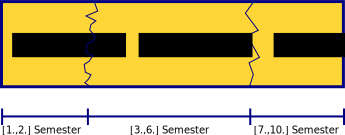
\includegraphics{phasen}}}
\end{center}

\begin{kcmt6XX}

Neue version!

Die Anforderung an die Gestaltung des Angebots eines Studiengangs schlie"st
grunds"atzlich zwei Forderungen ein: gen"ugend "`fachliche Breite"' anzubieten
um eine gute Basis zu schaffen, sowie die M"oglichkeiten eine gewisse
"`fachliche Tiefe"' zu erreichen -- sowohl vor als auch speziell in der Vertiefungsphase
des Studiums.

Hier konkrete Forderungen zu stellen ist uns nicht im Konsens m"oglich, und dies
zeigt auch schon die Freiheit, die den Hochschulen in der Gestaltung ihrer Studieng"ange
nat"urlich vorbehalten bleiben soll. Andererseits k"onnen unsere Forderungen besser
durch folgendes Modell dargestellt werden.

\paragraph{Modell} Dem Modell liegt folgender Gedanke zu Grunde: "`Gehen wir einmal davon
aus, dass F"acher bzw. Themengebiete eine Metrik h"atten."' Als Beispiel sei hier eine
"`Messung"' der Distanz zwischen bspw. "`reiner"' und "`angewandter"' Mathematik, oder
eine zwischen "`Lineare Algebra I"', "`Lineare Algebra II"' und "`Analysis"' genannt. Durch diese Metrik
lassen sich Umgebungen finden, die verschiedene Themengebiete der Mathematik umfassen
und sich thematisch "`eng"' gruppieren. Weiterhin entstehen durch behandelte, "`entfernte"'
Themengebiete neue "`Dimensionen"'. Folgendes Beispiel soll dies verdeutlichen:

\begin{center}
\framebox{\resizebox{.75\textwidth}{!}{\includegraphics{dimensionen}}}
\end{center}

Dieses Beispiel zeigt eine m"ogliche Grundausbildung, welche f"ur gen"ugend "`fachliche
Breite"' sorgt, sowie mehrere verschiedene potentielle Zuk"unfte f"ur den Studierenden
-- an dieser Hochschule oder anderswo -- mit Schwerpunkten in verschiedenen Bereichen.

Der Nullpunkt stellt hier das erworbene Wissen innerhalb des Studiengebietes dar.
Mit der Zeit, w"ahrend die Studierenden durch die verschiedenen Phasen ihres Studiums
fortschreiten, entwickeln sie sich auf den verschiedenen Skalen (Dimensionen)
vorw"arts. Hier kommt auch wieder die Konzeption der Studieng"ange ins Spiel, speziell
inwiefern verschiedene Skalen angeboten werden, wieviele verpflichtend und optional
sind, wie weit sich Studierende weiterentwickeln k"onnen etc.

Mit diesen beiden Modellen vor Augen k"onnen die Minimalstandards formuliert werden.
Diese schlie"st auch eine gewisse Mobilit"at, Autonomie und Engagement
der Studierenden mit ein; dieses wird jedoch von der Hochschule sowohl erm"oglicht
als auch gef"ordert.

Es ist nicht Aufgabe der Minimalstandards einen F"acherkatalog bzw. curriculare
Vorschl"age darzubieten. Dies geschieht stattdessen im Rahmen der Hochschulen und
ihrer Koordination untereinander.

\begin{kcmt62}
\begin{komacmt62}
\begin{eqnarray*}
	dim(V) \geq & n \\
	n > & 1 \\
	Geg. \epsilon > & 0:\\
	\forall  v \in V & \exists u \in V_\epsilon(v) \backslash \{v\}
\end{eqnarray*}

Diese Formeln hier sind aus dem Dokument gewandert weil sie f"ur zuviel
Verwirrung sorgen. Zwar l"a"st sich die Anforderung an den Studiengang
so zweifelsfrei formulieren, andererseits aber ist diese Formulierung
nicht leicht verst"andlich.
\end{komacmt62}
\end{kcmt62}

\begin{kcmt62}
\begin{komacmt62}
Folgendes wird durch die Arbeit von Karin \& Co. ersetzt:

Das hei"st es werden mindestens zwei Themengebiete der Mathematik an der Hochschule
abgedeckt. Weiterhin existiert eine maximale Spanne zwischen den verwandten
Gebieten, was bedeutet das eine kontinuierliche Weiterentwicklung der F"ahigkeiten
und Kenntnisse der Studierenden im ausgew"ahlten Gebiet stattfindet -- die Vorlesungen
entwickeln sich sozusagen "`stetig"' und bauen aufeinander -- im Sinne der Skala dieser
"`Dimension"' der Mathematik -- auf.
\end{komacmt62}
\end{kcmt62}

\end{kcmt6XX}

\section{Diversit"at und Spezialisierung}

Die Anforderung an die Gestaltung des Angebots eines Studiengangs schlie"st grunds"atzlich zwei Forderungen ein: 
\begin{enumerate}
	\item Gen"ugend "`fachliche Breite"' anzubieten, um eine gute Basis zu schaffen.
	\item Die M"oglichkeiten eine gewisse "`fachliche Tiefe"' zu erreichen -- sowohl vor als auch speziell in der Vertiefungsphase des Studiums.
\end{enumerate}

Um die abstrakten Begriffe "`fachliche Tiefe"' und "`fachliche
Breite"' fassen zu k"onnen, verwenden wir ein Modell zur Einordnung
der verschiedenen Lehrveranstaltungen bzw. zur Beschreibung ihrer
Beziehung untereinander.  Eine Veranstaltung l"asst sich mindestens
einem Bereich (Richtung) der Mathematik zuordnen. Diese Richtungen
spannen als Achsen den Raum der m"oglichen Veranstaltungen auf.
Hierbei entspricht der Nullpunkt dem Wissensstand eines Studienanf"angers.
Die Entfernung einer Veranstaltung vom Nullpunkt ist ein Ma"s f"ur
die fachliche Tiefe, die sie einem Studenten verleiht.

\begin{center}
\textbf{Ein Beispiel}\\
\framebox{\resizebox{.75\textwidth}{!}{\includegraphics{dimensionen}}}
\end{center}

Im Folgenden werden die Minimalstandards der Diversit"at und Spezialisierung formuliert:
\begin{enumerate}
\item Eine Hochschule bietet mindestens zwei unterschiedliche fachliche Richtungen innerhalb der Mathematik an.

\item Wenn eine (weiterf"uhrende) Veranstaltung Wissen voraussetzt,
welches "uber den Wissensstand eines Studienanf"angers hinausgeht,
wird zeitnah eine Veranstaltung angeboten, die dieses Wissen zuvor vermittelt.

\item In mindestens zwei der angebotenen Richtungen gibt es gen"ugend
weiterf"uhrende Veranstaltungen, so dass eine kontinuierliche
Weiterentwicklung der F"ahigkeiten und Kenntnisse des Studenten
stattfindet.

Hierzu geh"ort: Er lernt in mindestens zwei Richtungen seiner Wahl
Zusammenh"ange seines Faches zu "uberblicken und selbstst"andig
mathematische Methoden auszuw"ahlen und sachgerecht anzuwenden.
Des Weiteren lernt er, sich selbstst"andig in verwandte neue Themen
einzulesen und diese nachzuvollziehen.
\end{enumerate}

Diese Forderungen gehen auch von einer gewissen Mobilit"at, Autonomie
und einem Engagement des Studenten aus; dieses wird von
der Hochschule sowohl erm"oglicht als auch gef"ordert.

Es ist nicht Aufgabe der Minimalstandards, einen F"acherkatalog bzw.
curriculare Vorschl"age darzubieten. Dies geschieht stattdessen im
Rahmen der Hochschulen und ihrer Koordination untereinander.




\section{Erste Studienphase}

Der
Student kommt an die Hochschule und durchl"auft zun"achst eine Orientierungsphase.
W"ahrend dieser gew"ohnt er sich an das Lern- und Arbeitsniveau der Hochschule und
findet sich fachlich, sowohl was die Affinit"at zu etwaigen pers"onlichen Schwerpunkten
als auch was das gesamte mathematische Angebot anbelangt, in der Hochschule ein.

In der ersten Phase des Studiums wird der Student an das Fachgebiet herangef"uhrt.
Durch Schaffen einer soliden Basis wird sowohl die Vertiefung ausgew"ahlter Themen
erm"oglicht als auch die Autonomie gest"arkt, indem der sp"ateren Auswahl der
Spezialthemen ein solides Fundament unterstellt wird.

Hierbei wird auch auf Schwankungen bei den Vorkenntnissen der Studenten
eingegangen, d.h. nach Abschluss der ersten Studienphase sind eventuell 
vorhandene M"angel erkannt und ausgeglichen.

In der ersten Phase des Studiums wird noch keine Vertiefung erwartet; hier werden
die Richtungen geschaffen, und erste Schritte innerhalb dieser gemacht.
Der Student wird hierbei mit den an der Hochschule behandelten Themengebieten
vertraut gemacht (siehe Vorlesungen, Seite \pageref{vorlesung:anforderungen}).

Nach dieser Phase kann ein Student mit m"oglichst geringem Aufwand die Hochschule
bzw. den Studiengang wechseln.


\section{Zweite Studienphase}

Der Student hat inzwischen ein fachliches Basisniveau erreicht und
kann schon erkennen, welche Vertiefungsm"oglichkeiten an der eigenen Hochschule angeboten
werden und wie auf diese hingef"uhrt wird.
Im Rahmen dieser Studienphase wird er zur Auswahl der Schwerpunkte bef"ahigt. 

In der zweiten Studienphase finden in ausgew"ahlten Richtungen Vertiefungen statt,
eine weitere Spezialisierung des Studenten wird vorbereitet. Um den Studenten Vertiefungen in verschiedene Richtungen zu erm"oglichen, unterst"utzt die Hochschule
in dieser Phase auch Hochschulwechsel.
Bei diesen werden bereits erbrachte gleichwertige Leistungen anerkannt.
Bei abweichenden Studieng"angen muss
aber auch der Student Aufwand einplanen um sich dem Curriculum der neuen
Hochschule anzupassen.

Ein Studienwechsel wird durch die Hochschule zumindest soweit unterst"utzt, dass auf Anfrage eines Studenten Informationen "uber die gew"unschte Vertiefung an anderen Hochschulen bereitgestellt werden. Die Hochschule, an die gewechselt wird, stellt auf Anfrage klar, welche Leistungen anerkannt werden und welche Leistungen nachzuholen sind.

In dieser Phase wird sowohl die fachliche Breite als auch die fachliche Tiefe gef"ordert.

\section{Dritte Studienphase}

Ein Student der dritten Phase kann schon einen ersten Hochschulabschluss besitzen
und ist in der Lage, selbstst"andig wissenschaftlich zu arbeiten sowie autonom seine Spezialisierung
auszuw"ahlen und voranzutreiben. Nach der dritten Phase besitzt er die F"ahigkeit,
mathematische Methoden und wissenschaftliche Erkenntnisse selbstst"andig anzuwenden.

Hierbei wird dem Studenten erm"oglicht, sich in den von ihm gew"ahlten Richtungen
weiter zu vertiefen.

Ist keine dritte Phase vorhanden, kann mit Abschluss der zweiten Phase ohne Verl"angerung der Gesamtstudienzeit die dritte Phase an einer anderen Hochschule absolviert werden. Informationen "uber geeignete Hochschulen sind dem Studenten rechtzeitig bekannt zu geben.


\section{Kontinuit"at}

Ein Studium ist, gleich welche der angebotenen Richtungen der Student w"ahlt, 
in der Regelstudienzeit absolvierbar.

\begin{kcmt}\begin{komacmt}
Wenn der Student eine bestimmt Vertiefungsrichtung, die an der Hochschule
angeboten wird, studieren m"ochte, so kann er dies unabh"angig von seinem Studienbeginn 
tun. z.B. BA-Arbeit, auf der Zyklus nicht eingestellt war. Vorlesungszyklen, die nicht 
regelm"a"sig angeboten werden. Die Wdh- Rate der Zyklen darf die Gesamtstudienzeit nicht beeinflussen
\end{komacmt}\end{kcmt}

Aufeinander aufbauende Studieng"ange sind in Regelstudienzeit absolvierbar,
insbesondere wirkt sich der "Ubergang von einem Studiengang in einen darauf aufbauenden Studiengang nicht notwendig verl"angernd 
auf die Gesamtstudienzeit aus.

\begin{kcmt}\begin{komacmt}
Damit sollen eventuelle L"ucken vermieden werden, die sich aus der strukturellen 
Eigenschaften des BA-Stud. ergeben. Kern, BA + MA = 10 Semester regel. Problem: 
BA-Arbeit nicht in Zyklen eingeplant.
\end{komacmt}\end{kcmt}

Die Umsetzung der Studienordnung, insbesondere das Vorlesungsangebot und die 
Pr"ufungsordnungen, ist so flexibel gestaltet, dass Abweichungen vom planm"a"sigen 
Studienverlauf das Gesamtstudium nicht unverh"altnism"a"sig verl"angern. 
Speziell zieht ein Ausfall von einem Semester h"ochstens eine Studienzeitverl"angerung 
von zwei Semestern nach sich.

\begin{kcmt}\begin{komacmt}
Ausfallgr"unde: Krankheit, Unfall, Auslandssemester, private Probleme, sonst. Zielt wieder auf Zyklen ab.


Allgemein sehen wir es als schwierig an, wenn auf die bisherige Zyklen-Anordnung eine 
BA-MA Struktur ohne Anpassung gest"ulpt wird (Stichwort Aussetzen von einem Semster 
wg. BA-Arbeit und weiterlaufen des Zykluses) Vorlesungszyklen o."a m"ussen an die 
strukturellen Gegebenheiten angepasst werden. 
\end{komacmt}\end{kcmt}

\section{Teilzeitstudium / Studieren mit Kind}

Ein Beispielstudiengangsverlauf ist angegeben, bei dem die maximale Arbeitsbelastung 
pro Semester ein gewisses H"ochstma"s (Richtlinie: Alleinerziehendes Elternteil) nicht 
"ubersteigt. Dabei sind keine besonderen Vorkenntnisse gefordert, insbesondere ist auch
die Studiengeb"uhrensituation beachtet. Unter Ber"ucksichtigung dieser Rahmenbedingungen
entsteht dem Studenten bei Einhaltung dieses Beispielstudienverlaufs kein finanzieller
Nachteil.

\begin{kcmt}\begin{komacmt}
Ein Teilzeitstudium muss in angemessener Zeit schaffbar sein. Das Verh"altnis 
Semesterbelastung / Studienl"ange soll ungef"ahr gleich bleiben. 
Hier m"ussen noch konkrete Zahlen gefunden werden. 
\end{komacmt}\end{kcmt}

\section{Pr"ufungen}

Bei benoteten Modulen wird zu Beginn der einzelnen Veranstaltung(en) die Bewertungsmethode 
transparent gemacht. Insbesondere gilt f"ur Module, die mehrere Veranstaltungen 
oder Submodule beinhalten, dass dies mit Beginn der ersten Veranstaltung vorgestellt wird.
Mit Einverst"andnis aller Teilnehmer kann das System auch w"ahrend des Moduls ge"andert werden. 

Wenn das Nichtbestehen einer Pr"ufung einen Studienausschluss zur Folge hat, so 
wird dem Studenten die M"oglichkeit gegeben, die Pr"ufung mindestens zweimal
zu wiederholen. Dem Studenten wird die M"oglichkeit gegeben, die Pr"ufung 
so zu wiederholen, dass es zu keiner Verz"ogerung in seinem Studienverlauf kommt. 
Andererseits wird dem Studenten die M"oglichkeit gegeben, die Pr"ufung entweder
z"ugig zu wiederholen oder vor einer erneuten Pr"ufung pr"ufungsrelevante Veranstaltungen
erneut zu besuchen.

\begin{kcmt}\begin{komacmt}
Diese beiden Versuchen schlie"sen sich gegenseitig nicht aus.
\end{komacmt}\end{kcmt}

Werden Pr"ufungstermine vorgegeben, so sind diese mindestens einen Monat im voraus
anzuk"undigen.
\begin{kcmt}\begin{komacmt}
	Dies zielt auf zentrale Klausuren und nicht 
	auf individuelle Absprachen ab

	Wir beschr"anken uns erstmal nur auf Pr"ufungen, die im negativen Fall 
	einen Ausschluss vom Studium zur Folge haben.  Unsere Forderungen implizieren 
	insbesondere, das bei Modulen, deren Bestehen f"ur weitere Module Vorausssetzung 
	ist, ggf. mehr Wiederholungstermine angeboten werden m"usssen. 
\end{komacmt}\end{kcmt}

\subsection{Schriftliche Arbeiten}

Schriftliche Arbeiten werden von einem Studenten eigenst"andig angefertigt.
Bei einem umfangreichen Thema kann dieses auch entsprechend von mehr Studenten gemeinsam bearbeitet werden.
Jeder Student wird von einer fachlich kompetenten Person betreut.
Der Betreuer ist zu mindestens einem monatlichen pers"onlichen Gespr"ach bereit.
Zus"atzlich ist er f"ur kurze Nachfragen jederzeit erreichbar und antwortet auf diese innerhalb einer Woche.

Das zu behandelnde Thema wird zu Beginn der Arbeit festgelegt.
Die vom Studenten ge"au"serten Interessen werden bei der Vergabe des Themas ber"ucksichtigt.
Auf Wunsch des Studenten erfolgt die Vergabe des Themas so rechtzeitig, dass das Studium nicht unn"otig verl"angert wird.
Der Umfang des Themas wird so gew"ahlt, dass die Arbeit im daf"ur vorgesehenen Zeitrahmen fertiggestellt werden kann.


\section{Kontinuit"at der Studienordnung}

Jedem Studenten, der in einer Studienordnung beginnt, ist es m"oglich, in dieser sein Studium auch abzuschlie"sen.

Dies gilt insbesondere, wenn die Studienordnung ausl"auft.
In diesem Fall hat er f"ur das erfolgreiche Abschlie"sen des Studiums ab dem Zeitpunkt, zu dem keine Neueinschreibung gem"a"s dieser Studienordnung mehr m"oglich ist, Regelstudienzeit plus ein Jahr Zeit.
Sofern eine neuere Studienordnung existiert, ist es dem Studenten jederzeit m"oglich, auf diese wechseln.
Die bereits erbrachten Leistungen werden gem"a"s klar formulierten "Ubergangsregelungen (z.B. einer "Aquivalenzliste) anerkannt.

\begin{kcmt}\begin{komacmt}
	Gesetzliche Vorschrift nochmal erw"ahnen. Wenn ich in einer Studienordnung 
	beginne, musss ich mit dieser auch beenden k"onnen. Insbesondere, wenn es ein wenig l"anger dauert.
\end{komacmt}\end{kcmt}

\begin{stilltodo}
\section{Autonomie}

{\Large{Still To Do.}}
\end{stilltodo}

\section{Freiheit des Lernens}

Der Student ist selbstst"andig und "ubernimmt Eigenverantwortung. Die Hochschule
unterst"utzt ihn in der Freiheit, seinen Studienverlauf selbst zu gestalten.
Das umfasst sowohl die Anordnung der Veranstaltungen als auch die Wahl der Methodik
und Sozialform des Lernens, wie z.B. Autodidaktik.

Grunds"atzlich widerspricht Anwesenheitspflicht bei Veranstaltungen dem Gedanken
der Freiheit des Lernens, einzige Ausnahme k"onnen Seminare darstellen. Wenn Zulassungsvoraussetzungen
zur Pr"ufung einer Veranstaltung existieren, dann sind diese nur innerhalb dieser
Veranstaltung zu erbringen.

Die Wahl des Zeitpunkts des Studienabschlusses ist dem Studenten "uberlassen.

\begin{kcmt}\begin{komacmt}
	Gegenst"uck zur Verschulung. Selbstverantwortung der Studierenden. Wahlm"oglichkeiten alleine reichen nicht aus.
\end{komacmt}\end{kcmt}

\section{Orientierung an den Interessen der Studierenden}
Dem Studenten wird die M"oglichkeit gegeben, das Veranstaltungsangebot mitzugestalten. 
Dies bedeutet, dass in allen Gremien, welche Studien- und Pr"ufungsordnungen oder die 
Vorlesungsverzeichnisse beschlie"sen, Studenten mit Stimmrecht vertreten sind. Diese sind
durch die Fachschaft zu w"ahlen.

\begin{kcmt}\begin{komacmt}
Er muss die M"oglichkeit bieten, Fehlendes aus einem BA Studium nachzuholen -> Kontinuit"at
\end{komacmt}\end{kcmt}

\begin{kcmt}\begin{komacmt}
\paragraph{Noch fehlend}
\begin{itemize}
 \item fachliche Breite definieren
 \item Autodidaktisches Studium
 \item Beispielstudienverl"ufe
\end{itemize}
\end{komacmt}\end{kcmt}

\chapter{Veranstaltungsformen}

\begin{kcmt}\begin{komacmt}
\textbf{M"ogliche Formen}...

\begin{itemize}
	\item Vorlesung: (definiert).
	\item "Ubung: (definiert).
	\item Tutorium: (definiert).
	\item Praktika: (Anforderungen bei Pflichtpraktika unter Infrastruktur zu finden).
	\item Seminar: (definiert)
	\item Fragestunden/Konversatorische Stunden (Braucht's nicht: T + "U + geile Studis = kein Problem).
	\item Nachhilfe (Braucht's nicht: T + "U + geile Studis = kein Problem).
	\item Vorkurs/Orientierung (kein Minimalstandard, n"aheres dazu siehe unten in den Kommentaren)
	\item Service (siehe "`Service"', S.~\pageref{l.service})
\end{itemize}

\end{komacmt}\end{kcmt}

\section{Globale Forderungen}

\begin{itemize}
\item	Alle Veranstaltungen der Hochschule sind frei zug"anglich. 
\begin{kcmt}\begin{komacmt}
	Mit "`frei zug"anglich"' ist gemeint, dass ein Student jede Veranstaltung zumindest als Gasth"orer besuchen darf. Eine aktive Teilnahme kann ggf. bei Veranstaltungsformen wie Seminaren, Praktika auf eine feste Teilnehmerzahl beschr"ankt sein. (neu: Graz KoMa 65)
\end{komacmt}\end{kcmt}

\item	Alle Lehrenden bieten w"ahrend ihrer Lehrveranstaltungen und der Betreuung von Pr"ufungsleistungen eine w"ochentliche Sprechstunde an oder zumindest die M"oglichkeit einen Termin innerhalb einer Woche zu vereinbaren. Sofern der Lehrende f"ur mehr als eine Woche nicht erreichbar ist, muss ein alternativer Ansprechpartner vorhanden sein.

\begin{kcmt}\begin{komacmt}
	(Karlsruhe) Im Teil-AK trat die Frage auf, ob eine garantierte w"ochentliche Sprechstunde
	nicht schon den Rahmen "`Minimal"' sprengt. Reicht nach Vereinbarung
	innerhalb einer Woche nicht schon aus?

	(Karlsruhe: Robert) ist eine w"ochentliche Sprechstunde nicht eine Einschr"ankung?
	Quasi gefordert, es reicht wenn der Prof nur zur Sprechstunde erreichbar ist?

	(Graz) Mit "`Termin innerhalb einer Woche vereinbar"' verstehen wir, dass die Terminabsprache nicht l"anger als eine Woche dauert, der Termin danach aber zeitnah stattfinden muss.
\end{komacmt}\end{kcmt}

\item	Die Lehrenden bzw. Betreuenden sind fachlich und didaktisch kompetent.
	
\item	Es werden nicht nur Probleml"osungen vermittelt. Es wird auch gelehrt, Probleme zu l"osen.

\begin{kcmt}\begin{komacmt}
	(Fritz) Hierbei ist gemeint, da"s nicht nur das reine Reproduzieren von bekannten
	L"osungen ("uberhaupt) eine Lehre der Mathematik auszeichnet, sondern das
	Vermitteln einer mathematischen Denke. Hierzu ist es absolut notwendig,
	da"s neben Probleml"osungen eben auch gelehrt wird Probleme zu l"osen.
\end{komacmt}\end{kcmt}
	
\item	Vom Studenten wird erwartet, den Stoff der vorhergehenden Lehrveranstaltung durch
	Aufbereitung ausreichend verinnerlicht zu haben, um ein kontinuierliches Voranschreiten
	im Stoff zu gew"ahrleisten. Der Zeitaufwand daf"ur "uberschreitet dabei das 
	eineinhalbfache der f"ur die Vorlesung vorgesehenen Zeit nicht.

\item	Die hier vorgestellten Veranstaltungsformen beziehen sich auf alle Phasen des Studiums.
	Der Gebrauch des Begriffes "`Basisveranstaltung"' beschreibt die Veranstaltungen der
	ersten Studienphase.
	
\item	Alle Veranstaltungen werden jedes Semester evaluiert, sofern die Anonymität der Befragten gewährleistet bleibt. Die Ergebnisse sind f"ur die Studenten in ausgewerteter Form zug"anglich.

\begin{kcmt}\begin{komacmt}
	Details zur Evaluation kommen anderswo her und ist auch von der Veranstaltungsform abh"angig.
	Nicht how-to-eval vorschreiben sondern da"s\dots

	(Graz) F"ur Details verweisen wir auf die Resolution der KoMa~64 zu Evaluationen.
\end{komacmt}\end{kcmt}

\item	Nach dem bestandenen ersten Studienabschnitt wird davon ausgegangen, dass alle Studenten 
	sich auf etwa gleichem Niveau befinden. Hierbei wird auch auf Schwankungen bei den
	Vorkenntnissen der Studenten eingegangen, d.h. das erreichte Niveau ist unabh"angig
	vom Zeitpunkt des Studienbeginns. Eventuell vorhandene und erkannte M"angel des Studenten
	werden durch zus"atzliche Veranstaltungen oder Hilfestellungen, wie z.\,B. "Ubungen, Zusatzmaterial ausgeglichen.

\item	F"ur die Mehrheit der Studenten gen"ugen 50 Stunden Arbeitsaufwand pro Woche, um das Studium in Regelstudienzeit erfolgreich abzuschlie"sen.
	Der Arbeitsaufwand beinhaltet sowohl die Zeit f"ur den Besuch von Veranstaltungen als auch f"ur die Nachbereitung, Hausaufgaben, schriftliche Arbeiten und "ahnliches.
\begin{kcmt}\begin{komacmt}
	x bestimmen. (Fritz) Hinweis: Eigentlich gibt es ECTS, nach derem System basierend auf
	Semesterwochenstunden "`ausgerechnet"' werden k"onnte, wieviel Wochenarbeitsstunden auf
	"Ubungsaufgaben entfallen k"onnen. Der Sinn hier ist eine Begrenzung nach oben, und es
	ist fraglich, ob die bearbeitende Gruppe einen Konsens mit dem ECTS findet.
\end{komacmt}\end{kcmt}
\end{itemize}

\section{Vorlesung}

\subsection{Definition} 
	Eine Vorlesung ist eine regelm"a"sige und fortlaufende Unterrichtsveranstaltung, die von einem
	Professor, Lehrbeauftragten oder wissenschaftlichen Mitarbeiter im Vortragsstil gehalten wird.


\subsection{Ziel} 
	Ziel von Vorlesungen ist die Vermittlung fachlichen Wissens auf theoretischer Basis. 

\subsection{Anforderungen} \label{vorlesung:anforderungen}

\begin{itemize}
	\item Der Lehrstoff ist inhaltlich und visuell so aufbereitet, dass die Studenten
	mehrheitlich nicht "uberfordert sind.
\begin{kcmt}\begin{komacmt}
	Hier betreten wir ein Minenfeld, das Spannungsfeld "`Qualit"at der Vorlesungen"' $\Leftrightarrow$ "`Qualit"at
	der Studierenden"'. Man k"onnte die Anforderung, Zwei Drittel der Studierenden nicht zu verlieren, auch
	dadurch erf"ullen, indem der Stoffumfang erheblich gek"urzt wird. Ref. Fachliche Breite und Tiefe :)

	Anders gesagt, der Stoff mu"s gleich bleiben bzw. der Stoffumfang sollte nicht gek"urzt werden
	um hier etwas zu erreichen.

	Weiterhin macht die Messung ein Problem: Gerade zu Beginn des Studiums sind einige Studierende
	noch anwesend, die f"ur das Studium (allgemein oder das der Mathematik) ungeeignet sind. In dieser
	inhomogenen Menge (bzgl. des vorherigen Ausbildungs- und Leistungsstand) eine Messung durchzuf"uhren
	f"uhrt hier am Ziel vorbei.

	Anmerkung aus dem Plenum: diese "`Messung"' kann ja auch von den betreuenden Studierenden
	durchgef"uhrt werden ($\rightarrow$ "Ubungsgruppenleiter, Mentor, \dots).
\end{komacmt}\end{kcmt}
	\item Durch Bereitstellung und/oder Verweise auf begleitende Lehrmaterialien ist es dem Studenten
		m"oglich das Lernziel auch autodidaktisch zu erreichen sowie in der Vorlesung angeeignetes Wissen weiter zu
		vertiefen.
	\item Eine Vorlesung wird bei Basisveranstaltungen grunds"atzlich von "Ubungen und/oder Tutorien begleitet. Das Verh"altnis der Stundenzahl von "Ubungen/Tutorien zur Vorlesung betr"agt mindestens 1:2.
\begin{kcmt}\begin{komacmt}
	Plenum: "`Braucht wirklich jede Vorlesung eine "Ubung?"' -- Die Antwort ist nat"urlich "`nein"'.
	\emph{Aber}: Wenn "Ubungen angeboten werden (und an anderer Stelle wird ja explizit f"ur Basisvorlesungen
	"Ubungen verlangt). Hier sollte die Formulierung wohl noch "uberarbeitet werden.
\end{komacmt}\end{kcmt}
	\item Zur Kl"arung fachlicher Fragen w"ahrend der Veranstaltung ist ein gewisses Ma"s an Interaktivit"at gegeben. Hierbei werden Thematik und Gruppengr"o"se ber"ucksichtigt. 
	\item Der Vortrag wird fachlich korrekt und sprachlich gut verst"andlich gehalten und ist didaktisch hochwertig.
	\item Eine sich durch das gesamte Semester ziehende Struktur des Lehrstoffes ist klar vom Studenten erkennbar.
	\item Um einen hohen Vernetzungsgrad zwischen den Vorlesungen zu erreichen, gibt es fachliche Einordnungen der Themen und Ausblicke auf weiterf"uhrende Veranstaltungen. 
\end{itemize}

\begin{kcmt}\begin{komacmt}
Nat"urlich sollen alle Veranstaltungen in einer Sprache gehalten werden, der mehrheitlich
die Studenten folgen k"onnen, dies erscheint uns jedoch als selbstverst"andlich.
\end{komacmt}\end{kcmt}



\section{"Ubung/Tutorium}

\begin{kcmt}\begin{komacmt}
	Eine Definition dieser beiden Veranstaltungsformen war notwendig geworden, da sich
	gezeigt hat, da"s unter "`"Ubung"' bzw. "`Tutorium"' an verschiedenen Hochschulen
	Verschiedenes verstanden wird. Momentan ist die Definition noch so gefa"st, da"s
	das Konsens-Verst"andnis (Der Betreuer der "Ubungen ist fachlich h"oher qualifiziert
	als der des Tutoriums, welcher "ublicherweise ein Studierender ist) der Veranstaltungen
	\emph{beide} umfa"st. Das kann sich noch "andern.
\end{komacmt}\end{kcmt}

\subsection{Definition} 

	Eine "Ubung bzw. ein Tutorium ist eine Kleingruppe von allerh"ochstens 30 Studenten, die von einem geeigneten 
	Lehrverantwortlichen betreut wird und notwendigen Stoff und "Ubungsaufgaben behandelt.

\subsection{Ziel} 

	In einer "Ubung bzw. einem Tutorium wird die in der Vorlesung vermittelte Theorie angewandt und wiederholt
	sowie erlernter Stoff gefestigt. "Ubungen und Tutorien besch"aftigen sich mit der Konstruktion von Beispielen 
	und L"osungen von Aufgabenstellungen.

\begin{kcmt}\begin{komacmt}
Der Gedanke hierbei ist, dass "Ubungen sowohl L"osung, L"osungen und auch -- bei "`interessanten"'
Themen mehrere L"osungsm"oglichkeiten aufzeigen und "`vorexerzieren"' sollen.
\end{komacmt}\end{kcmt}

\subsection{Anforderungen}

\begin{itemize}
	\item Die Veranstaltungen sind mit den zugeh"origen Vorlesungen eng verkn"upft.
	\item Der Schwerpunkt liegt auf Interaktivit"at.
	\item Die "Ubungsaufgaben zu den Basisvorlesungen werden korrigiert und kooperativ gel"ost, w"ahrend es bei anderen
		Vorlesungen akzeptabel ist auf vorhandene L"osungen zu verweisen und die autodidaktischen F"ahigkeiten
		der Studierenden zu fordern und f"ordern.
\begin{kcmt}\begin{komacmt}
	In h"oheren Semestern kann man mehr von Studierenden verlangen. Das bedeutet unter anderem
	auch, da"s man von ihnen erwarten kann, da"s sie auch tiefergehende Themen autark aufarbeiten.
	Gleichzeitig soll der Studierende in diesem Proze"s unterst"utzt werden.
\end{komacmt}\end{kcmt}
	\item Im Gro"steil der Zeit sollte die Mehrheit der Studenten in der Lage sein, der "Ubung zu folgen und aktiv mitzuarbeiten.
	\item Zus"atzlich kann eine Global"ubung angeboten werden, die sich auf das Vorrechnen von Aufgaben konzentriert;
		hierbei ist die Gruppengr"o"se nicht beschr"ankt.
\begin{kcmt}\begin{komacmt}
	Dieser Bulletpoint sollte der letzte sein.

	Das Wort \emph{Zus"atzlich} soll hier ausdr"ucken, da"s diese Global"ubungen das oben
	angesprochene Verh"altnis von "Ubungen bzw. Tutorien zu Vorlesungen \emph{nicht} ber"uhren.
\end{komacmt}\end{kcmt}
	
\end{itemize}

\section{Seminar}

\subsection{Definition} 
	In einem Seminar tragen Studenten "uber ein vorher eigenst"andig aufbereitetes Thema vor. Dieses wird
	von einem fachlich kompetenten Lehrk"orper betreut.

\begin{kcmt}\begin{komacmt}
Lehrk"orper = Dozent, weitere Mitarbeiter die Vortr"age betreuen, "`alle, die etwas mit dem Seminar zu tun haben"' (und keine H"orer sind).
\end{komacmt}\end{kcmt}

\subsection{Ziel} 
	Ziel eines Seminars ist es, das eigenst"andige wissenschaftliche Arbeiten zu f"ordern
	und zur Pr"asentation von Ergebnissen zu bef"ahigen. Der Student entwickelt hierbei ein
	tiefergehendes fachliches Verst"andnis.

\begin{kcmt}\begin{komacmt}
"uben. trainieren. aneignen. Formulierungswahn!
\end{komacmt}\end{kcmt}


\subsection{Anforderungen}
\begin{kcmt}\begin{komacmt}
\paragraph{Brainstorm!} \begin{itemize}
	\item Kein Powerpoint! (tongue in cheek)
	\item Vortrag eines Studierenden 
	\item zur Verf"ugung stehende Zeit zur Vorbereitung
	\item Betreuung
	\item Anspruch des Themas
	\item Feedback -- M"oglichkeiten zur (anschlie"senden) Diskussion
	\item Gruppengr"o"se (klein)
	\item Umfang des Stoffes (moderat)
	\item (vorgeschlagen und gestrichen  war noch: ) aufeinander aufbauende Themen
	\item \dots
	\item Eigenst"andigkeit
	\item F"ahigkeit zur Pr"asentation
	\item wissenschaftlich Arbeiten
	\item tieferes VErst"andnis
	\item intensive BEsch"aftigung mit Thema
	\item Interaktion
	\item Zwischenfragen ( + Vorbereitung darauf )
	\item Stil
\end{itemize}
"`Bef"ahigung zur Pr"asentation"': Zusammenfassen, zeitlicher, stofflicher Rahmen.
Auswahl der Tiefe des Themas.
\end{komacmt}\end{kcmt}

\begin{itemize}
	\item Alle Vortr"age beziehen sich auf ein vorher bekanntgegebenes Rahmenthema.
	\begin{kcmt}\begin{komacmt}
		(Fritz) Oberthema durch Rahmenthema ersetzt.
	\end{komacmt}\end{kcmt}
	\item Unterschiedlicher Arbeitsaufwand ist vor Vergabe der Vortr"age bekannt und auf Wunsch anzugleichen.
	\item W"ahrend der Erarbeitungsphase stellt der Dozent einen Ansprechpartner f"ur R"uckfragen zur Verf"ugung.
	\begin{kcmt}\begin{komacmt}
		(Fritz) Nat"urlich kann der Dozent auch sich selbst zur Verf"ugung stellen. Eine Minimalforderung
		ist jedoch "`nur"' einen angemessenen Ansprechpartner vorgesetzt zu bekommen, der vor allem bei
		fachlichen Fragen weiterhelfen kann.
	\end{komacmt}\end{kcmt}
	\item Der Anspruch der Vortragsthemen korreliert mit der zur Verf"ugung stehenden Bearbeitungszeit. Diese
		betr"agt mindestens zwei Wochen.
	\begin{kcmt}\begin{komacmt}
		(Fritz) Also die Zeit die zur Bearbeitung zur Verf"ugung steht betr"agt zwei Wochen, nicht wir
		gehen von einer Arbeitslast von mindestens zwei Wochen aus. Die Formulierung ist noch etwas wacklig m.E.
	\end{komacmt}\end{kcmt}
	\item Die Vortragenden erhalten Feedback vom Dozenten sowie auf Wunsch auch vom Auditorium.
	\item Ein Thema wird maximal von drei Studenten bearbeitet; jeder am Seminar teilnehmende Student hat die M"oglichkeit, an einem Vortrag mitzuwirken und pr"asentiert mindestens eine halbe Stunde lang.
\end{itemize}


\begin{kcmt}\begin{komacmt}
	(Karlsruhe) Julia besteht auf $>1$ Studierende/Vortrag, pr"aferiert 3. 2 tragbar. $<2$ Veto. Fritz will einen Vortragenden pro Thema. Z"ahneknirschender Konsenes mit Verweis auf \emph{Minimal}standards hergestellt.

	(Karlsruhe) Eine Folgerung: Gruppengr"o"se beschr"ankt weil jeder drankommen k"onnen soll, max 2 Leute pro Vortrag $\Rightarrow$ bei X Vorlesungswochen ($X=10\ldots 16$) ergibt sich eine obere Grenze.
	
	(Graz) Erneute Diskussion: Ideale Lerngruppengr"o{"s}e liegt bei 2-3, wir haben eine Mindestvortragszeit von 30 min/Student. Damit ergibt sich bei 90 min Vortrag: max 3 Studenten. Mit Verweis auf \emph{Minimal}standards haben wir auf 3 Studenten abgeschw"acht.
\end{komacmt}\end{kcmt}


	\begin{kcmt}\begin{komacmt}

\section{Vorkurs}

	Wir haben uns entschieden, den Vorkurs zu streichen, weil die Tatsache, dass der Vorkurs nicht z.B. f"ur LinA oder Analysis als Voraussetzung verpflichtend sein darf bereits durch den Abschnitt Freiheit des Lernens abgedeckt ist.
	Falls ein ``Vorkurs'' direkt in der Liste der Voraussetzungen f"ur den Abschluss stehen sollte, so kann man ihn dann eben irgendwann besuchen, so bekloppt das sein mag.

\subsection{Definition}
Ein Vorkurs ist eine Veranstaltung, die darauf ausgelegt ist, vor dem Beginn des eigentlichen Studiums besucht zu werden.

\subsection{Anforderungen}
\begin{itemize}
\item Falls ein Vorkurs stattfindet, darf er nicht verpflichtend sein.
\end{itemize}

	\end{komacmt}\end{kcmt}

\chapter{Infrastruktur}
\thispagestyle{fancy}

\section{Generelles}

\begin{itemize}
\item Grundlegende Dinge, wie ausreichende
Beleuchtung, Heizung, Toiletten, Sitzm"oglichkeiten, Platz zum
Schreiben und auch Schreibmaterialien (z.B. Tafeln oder Whiteboards mit zugeh"origem Material) sind vorhanden.

\item Die Infrastruktur ist w"ahrend der Vorlesungszeiten f"ur den Studenten zug"anglich.

\item Alle R"aumlichkeiten sind barrierefrei zug"anglich.

\item Aufeinander folgende Pflichtveranstaltungen finden 
		nahe genug beieinander statt. Es ist also in der Zeit zwischen den 
		Veranstaltungen m"oglich,  von einem Veranstaltungsort zu dem der folgenden zu gelangen.

\item Geb"aude und R"aume sind deutlich 
		sichtbar (auch international verst"andlich) gekennzeichnet.
		An zentralen Stellen sind Pl"ane vorhanden.
\end{itemize}


\section{R"aume}

\subsection{Veranstaltungsr"aume}

\begin{kcmt}\begin{komacmt}
Vorlesungs- und Seminarr"aume unterscheiden sich nur in der Gr"o"se und 
werden deshalb nicht gesondert behandelt. Spezielle R"aume f"ur Tutorien u.~"a. 
werden hier nicht erw"ahnt, da diese nicht unbedingt erforderlich sind 
(Jede "Ubung kann auch in einem Vorlesungs-/Seminarraum stattfinden.). 
Wenn es extra "Ubungsr"aume g"abe, w"are die Anzahl der insgesamt 
ben"otigten R"aume gr"o"ser (kein Minimalstandard).
\end{komacmt}\end{kcmt}
\begin{itemize}
	\item F"ur jede Veranstaltung steht ein Raum zur Verf"ugung.
	\item Jeder Zuh"orer bekommt bei den Veranstaltungen einen daf"ur vorgesehenen Sitzplatz.
	\item Auch zu Sto"szeiten sind ausreichend Kapazit"aten an R"aumlichkeiten vorhanden.
	\item Die R"aume verf"ugen "uber eine Tafel, die so gro"s ist,
		dass bei einer f"ur alle Anwesenden lesbar gro"sen Anschrift gen"ugend Tafelfl"ache vorhanden ist, um den f"ur das Verst"andnis des aktuellen Themas notwendigen Kontext zu fassen.
	\item Die R"aumlichkeiten m"ussen die M"oglichkeit der Visualisierung per Beamer 
		und/oder Overheadprojektor bieten. Es gibt in jedem Raum eine Projektionsfl"ache. 
		Dazu ist jeder Raum (mindestens die H"alfte aller R"aume gleichzeitig) mit den ben"otigten Ger"aten versorgbar.
\begin{kcmt}\begin{komacmt}
	Es sind nicht zu wenig, weil fast nie alle R"aume gleichzeitig besetzt sind und auch
	f"ur viele Veranstaltungen kein Beamer / Overheadprojektor n"otig ist. Es sind nicht
	zu viel, da es nicht sein kann, da"s sich ein Vortragender in der Wahl der Visualisierung
	nach dem Vorhandensein von Beamer/Overheadprojektor richten mu"s.
\end{komacmt}\end{kcmt}
	\item In den R"aumen ist der Dozent "uberall zu verstehen,
		geeignete Hilfsmittel (z.B. ein Mikrofon) stehen bei Bedarf zur Verf"ugung.
	\item Es gibt Platz, um Jacken, Taschen usw. abzulegen.
\end{itemize}

\subsection{Computerr"aume}
\begin{itemize}
	\item Es gibt eine der Anzahl der Studenten angemessene Menge frei zug"anglicher Rechnerpl"atze.
\begin{kcmt}\begin{komacmt}
	Eine genauere Kl"arnung von "`zug"anglich"' wurde gew"unscht, aber auf eine Definition konnten wir uns noch nicht einigen. Es geht dabei z.B. um "Offnungszeiten, Wartezeiten, et al. Ein Vorschlag war, eine angemessene Anzahl an Rechnerpl"atzen dar"uber zu definieren, dass es Zeiten gibt, zu denen nicht gewartet werden muss.

	\paragraph{Gestrichene Formulierung:} \begin{itemize}
	\item Das Verh"altnis von Studierenden zu Rechnerpl"atzen gesamt unterschreitet 7:1 nicht.
	\end{itemize}

	"`Warum 7:1?"' -- Diese Zahl wurde aus der Situation an der Fachhochschule Regensburg,
	TU M"unchen und Chemnitz gefolgert. Die urspr"ungliche Forderung war hier mal 5:1.
	Das Plenum findet aber auch 10:1 akzeptabel. Hier stellt sich auch die Frage nach
	Me"sgr"o"sen allgemein: sollen sie minimal, maximal, exakt beschreiben? "`Wenn diese
	Zahl "uberschritten wird ist's \emph{definitiv} schlecht?"'

	Die neue Formulierung dr"uckt aus, da"s kleine Fakult"aten mit einer Anzahl von
	Rechner im Verh"altnis 10:1 deutlich zu wenig Rechner h"atten.
\end{komacmt}\end{kcmt}
	\item W"ahrend Veranstaltungen mit PC-Einsatz gibt es mindestens halb so viele Rechner wie Studenten.
	\item Die Rechner sind entsprechend der Richtung der Hochschule mit Software 
		ausgestattet (Computeralgebrasystem, Numerische Software, Statistikprogramm, \dots). 
		Ein Programm zum Anfertigen auch umfangreicherer mathematischer Texte ist installiert.
\begin{kcmt}\begin{komacmt}
	Diese Ausstattung ist nat"urlich einwandfrei lizensiert, legal erworben etc.
	Ob hier auch Lizenzen f"ur Spezialsoftware an Studenten herausgegeben werden
	wurde nicht explizit diskutiert (Rauschen aus dem Plena).
	Freeware bzw. Open Source Software sind nat"urlich auch erlaubt.
\end{komacmt}\end{kcmt}
	\item Die Rechner verf"ugen "uber einen Internetzugang. 
	\item Es gibt eine Druckm"oglichkeit h"ochstens zum Selbstkostenpreis. 
		Die Funktionsf"ahigkeit dieser ist immer gew"ahrleistet (Toner, Papier vorhanden).
	\item Es gibt eine M"oglichkeit zur Visualisierung bei Lehrveranstaltungen (z.~B. Beamer, Tafel...).
\end{itemize}

\subsection{Studentische Arbeitsr"aume}
\begin{itemize}
	\item F"ur den Studenten besteht die M"oglichkeit freie Kapazit"aten herauszufinden 
		(Raumbelegungsplan) und diese zu nutzen. 
	\item Es ist ein Ruhebereich vorhanden, in dem gearbeitet werden kann.
	\item Ein Student, der an seiner Abschlussarbeit arbeitet, hat immer Zugang zu einem Rechner. 
		(Es sollte immer mindestens ein Rechnerpool frei sein.)
	\item Studentische Arbeitsr"aume sind mit einer Tafel bzw. einem Whiteboard ausgestattet.
\end{itemize}


\section{Fachschaft}

Die Fachschaft ist ein Zusammenschluss von Studenten eines Faches zwecks gemeinsamer Interessenvertretung.
Die Fachschaft wird durch die Hochschule unterst"utzt.

\begin{kcmt}\begin{komacmt}
Es geht hier \emph{nicht} um die Aufgaben der Fachschaften.

\begin{itemize}
	\item Rechnerzugang inklusive Webspace \& Mail-Adresse(n)
	\item Kopierm"oglichkeit
	\item B"uroraum mit Telefon
	\item M"oglichkeit f"ur regelm"a"sige FS-Sitzungen
	\item Erm"oglichung der Herausgabe von Infomaterial
\end{itemize}
\end{komacmt}\end{kcmt}

Um eine effiziente Fachschaftsarbeit zu gew"ahrleisten, stellt die Hochschule der Fachschaft folgendes zur Verf"ugung:
\begin{itemize}
	\item einen B"uroraum mit Telefon, dessen Gr"o"se der Anzahl der Studenten angemessen ist,
	\item einen Rechnerzugang inklusive Webspace f"ur eine Fachschaftswebseite und
		eine E-Mail-Adresse sowie
	\item eine Kopierm"oglichkeit.
\end{itemize}

Au"serdem erm"oglicht die Hochschule der Fachschaft regelm"a"sige
Fachschaftssitzungen (durch Bereitstellen eines geeigneten Raumes) und die
Herausgabe von Infomaterial, z.\,B. den Druck eines regelm"a"sigen Infohefts, von Plakaten,
Flyern und "ahnlichem. 

\newpage
\section{Bibliothek}
Eine Bibliothek ist vorhanden und bietet mindestens folgende M"oglichkeiten:
\begin{itemize}
	\item ausreichende Recherchem"oglichkeiten (z.B. am Rechner)
	\item den Veranstaltungen zu Grunde liegende und vertiefende Literatur
	\item ein Kopierer
	\item Arbeitspl"atze
	\item Die wichtigsten Fachzeitschriften sind vor Ort vorhanden, die anderen 
		per Fernleihe beziehbar.
	\item Nicht vorhandene B"ucher sind per Fernleihe zu beziehen.
	\item Es findet regelm"a"sig eine "Uberpr"ufung des Bedarfs statt, 
		so dass bei h"aufig vergriffenen Werken der Bestand aufgestockt wird.
\end{itemize}

\chapter{Service}
\thispagestyle{fancy}
\label{l.service}

\begin{kcmt62}
\begin{komacmt62}
	Service bezieht sich nicht speziell auf einzelne Veranstaltungen, sondern
	aufs Studium allgemein. Wenn wegen Bachelor und Master die Mobilit"at
	zwischen Hochschulen und/oder L"andern steigt, ist die Beratung ein
	Minimalstandard!

\end{komacmt62}
\end{kcmt62}
\begin{kcmt}\begin{komacmt}
	\paragraph{Bearbeitete Punkte:}
	\begin{itemize}
		\item Studienberatung / Fachberatung
		\item Erstsemesterinformation
		\item Fachschafts-Service
		\item Auslandsangebot
	\end{itemize}

	\paragraph{Ausstehende Punkte:}
	\begin{itemize}
		\item Pr"a-Studierenden-Info
		\item Schulungen f"ur Studentische Hilfskr"afte (Tutoren etc.)
		\item "Offnungszeiten (Bibliothek, Sekretariat)
	\end{itemize}

	Service bezieht sich nicht speziell auf einzelne Veranstaltungen, sondern
	aufs Studium allgemein. Wenn wegen Bachelor und Master die Mobilit"at
	zwischen Hochschulen und/oder L"andern steigt, ist die Beratung ein
	Minimalstandard!
\end{komacmt}\end{kcmt}

\section{Studienberatung}

\begin{kcmt}\begin{komacmt}
\emph{Hochschulweite Studienberatung}
\begin{itemize}
	\item bei Fachfragen sofort \& richtig (Fachberatung) weiterleiten
	\item generellen "Uberblick bieten
\end{itemize}
\end{komacmt}\end{kcmt}

Es gibt eine hochschulweite Beratungszentrale, die kompetent ber"at und weiterleitet.
Das Beratungsangebot umfasst folgende Bereiche:
\begin{itemize}
	\item fachliche Beratung "uber die einzelnen Studieng"ange
	\item Studienfinanzierung
	\item Studienrechtsberatung
	\item Beratung f"ur
		\begin{itemize}
			\item behindertengerechtes Studium
			\item Studieren mit Kind
			\item ausl"andische Studenten
			\item Auslandsstudium
		\end{itemize}
\end{itemize}

Unter angemessener finanzieller und organisatorischer Unterst"utzung kann ein 
Teil der Beratungsverpflichtung an die organisierte Studierendenschaft abgetreten werden.

\begin{kcmt}\begin{komacmt}
	Das hei"st aber auch, dass falls Bereiche der Beratung an die
	Studierendenschaft abgetreten werden, muss die abtretende Stelle
	auch daf"ur Sorge tragen, dass die Beratung auch effizient
	durchgef"uhrt wird.
\end{komacmt}\end{kcmt}

\section{Fachberatung}

\begin{kcmt}\begin{komacmt}
\textbf{Fachberatung}
\begin{itemize}
	\item Studienplanung
	\item Pr"ufungsplanung
	\item "Uberblick "uber m"ogliche Studienvertiefung(en)
	\item Anerkennung von Leistungen von anderen Hochschulen
	\item Informationen zum Studienwechsel
\end{itemize}
\end{komacmt}\end{kcmt}

Die Fachberatung ist daf"ur zust"andig, dass ein Student sein Studium
zielgerichtet durchf"uhren kann. Sie muss insbesondere zu folgenden
Themen kompetent beraten k"onnen:
\begin{itemize}
	\item Studienplanung
	\item Pr"ufungsplanung
	\item Studienvertiefung(en)/Spezialisierung(en)
	\item g"angige Nebenf"acher
	\item Anerkennung von Leistungen, die an anderen Hochschulen erbracht wurden
	\item Studienwechsel, sowohl Wechsel des Studiengangs als auch der Hochschule
\end{itemize}

Insbesondere beinhaltet die Beratung auch das Aufzeigen eines Beispielstudienverlaufs.
Innerhalb der Vorlesungszeit ist eine Beratung sp"atestens eine Woche nach
Anfrage eines Studenten gew"ahrleistet. In der vorlesungsfreien Zeit
kann diese Frist auf allerh"ochstens drei Wochen verl"angert werden.

\section{Betreuung der Studienanf"anger}

Jeder Studienanf"anger wird vor Studienbeginn mit Hilfe eines Infoheftes und der M"oglichkeit einer pers"onlichen Beratung "uber sein zuk"unftiges Studium informiert.

\begin{description}
	\item [Beratung] Die persönliche Beratung bietet vor allem einen Ausblick "uber das Studium, informiert "uber Voraussetzungen und Fristen und leitet bei weiterf"uhrenden Fragen an die entsprechenden Beratungsstellen weiter.

	\item [Infoheft] Das Infoheft (digital oder gedruckt) beinhaltet mindestens folgende Punkte:
	\begin{itemize}
		\item Pflichtveranstaltungen des ersten Jahres 
		\item Kommentar zu Vorlesungen des ersten Semesters
		\item Wichtige Ansprechpartner bzw. Anlaufstellen (mit Telefonnummer,
			E-Mail, Raumnummer, Sprechzeiten wenn m"oglich)
		\item wichtige Termine (z.\,B. R"uckmeldungsfristen, Pr"ufungsanmeldungszeitr"aume)
		\item Infrastruktur (Lageplan, Rechnerzugang, "Offnungszeiten, Bibliothek)
	\end{itemize}

	\begin{kcmt}\begin{komacmt}
	Voraussetzungen \& Fristen: Was muss ich vor dem Studium noch leisten,
	wof"ur mich noch anmelden.
	\end{komacmt}\end{kcmt}
\end{description}

\section{Praktikum}

Falls in einem Studiengang ein Pflichtpraktikum vorgesehen ist, bietet die Hochschule eine Anlaufstelle f"ur Praktikumsbelange. Diese erm"oglicht eine zeitnahe Betreuung des Studenten. Insbesondere bietet sie regelm"a"sige Sprechzeiten an.

Die Anlaufstelle dient der Vermittlung von Praktikumsstellen. Sie bietet Informationen und Hilfestellung bei eventuellen Problemen. Dies umfasst Informationen rein organisatorischer Art wie auch praktikumsvorbereitende und praktikumsnachbereitende Informationen und Hilfestellungen.

Des Weiteren besitzt die Anlaufstelle Informationen zu eventuellen Fristen, Terminen oder Zulassungsvoraussetzungen und setzt Betroffene fr"uhzeitig dar"uber in Kenntnis.

\begin{kcmt}\begin{komacmt}
gel"oscht, weil in anderen Abschnitten bereits vorhanden

\section{Transparenz}
	\begin{itemize}
		\item "Uberblick "uber Vertiefungen in der Mathematik geben
		\item Was an meiner Hochschule, was wo anders
		\item Kooperation mit anderen Hochschulen
		\item Minimum "Uberblick auf Homepage mit Links
		\item besser Vortr"age, Ringvorlesung o.\,"a.
	\end{itemize}


Die Hochschule stellt jedem Studenten einen inhaltlichen "Uberblick "uber die m"oglichen
Vertiefungen in der Mathematik zur Verf"ugung. Hierbei sind die an dieser
Hochschule angebotenen Vertiefungen ausf"uhrlich dargestellt.

	Eine blo"se Aufz"ahlung reicht hier nicht.
	Wie kann das transportiert werden?
	\begin{itemize}
		\item Homepage
		\item Infoheft
		\item Vortr"age etc.
	\end{itemize}
\end{komacmt}\end{kcmt}

\section{Webseite}

Die Hochschule besitzt eine "offentlich zug"angliche, barrierefreie Webseite, "uber die mindestens folgende Informationen verf"ugbar sind:
\begin{itemize}
\item Aktuelle Pr"ufungsordnungen aller an der Hochschule existierenden Studieng"ange. Dazu geh"oren auch auslaufende Studieng"ange.

\item angebotene Lehrveranstaltungen inklusive Name des Dozenten, kurzer Beschreibung und etwaiger inhaltlicher Voraussetzungen

\item Liste der Lehrst"uhle und Professoren mit angegebener Kontaktm"oglichkeit

\item Verweis auf die Fachschaft und deren Webseite, sofern vorhanden

\item Verzeichnis der vorhandenen Servicestellen

\item wichtige Termine, wie zum Beispiel R"uckmeldefristen, Vorlesungszeiten, Pr"ufungsanmeldungszeitr"aume und -termine, Termine von Informationsveranstaltungen
\end{itemize}


\section{Auslandsangebot}

Ein Aufenthalt im Ausland ist in den Studienverlauf integrierbar.  Hierbei
unterst"utzt die Hochschule den Studenten bei der Wahl und dem Kontakt zu einer Gasthochschule.

Ein Student, der von einer ausl"andischen Hochschule kommt, wird bez"uglich
Visa und anderen Rechtsfragen, Wohnungssuche, Integration und f"ur ihn geeignete Veranstaltungen
beraten und unterst"utzt.


\newpage
\thispagestyle{empty}
~
\vfill
\begin{center}
\url{www.die-koma.org}
\end{center}

\end{document}
